\documentclass[12pt,titlepage]{article}
\usepackage[margin=1in]{geometry}
\usepackage{multicol}
\usepackage{graphicx}
\usepackage{fancyhdr}
\graphicspath{{./}}
\setlength\parindent{0pt}
\fancyhf{}
\rfoot{Page \thepage}

\begin{document}
\begin{titlepage}
	\centering
	\vfill
	{\bfseries\Large
		Joseph Morgan\\
		\large
		Homework 3\\
		\vskip2cm
		CISP440\\
	}
	\vfill
	\vfill
	\vfill
	\begin{figure}[h]
		\caption{My two perscriptions with the dates they were filled}
		\centering
		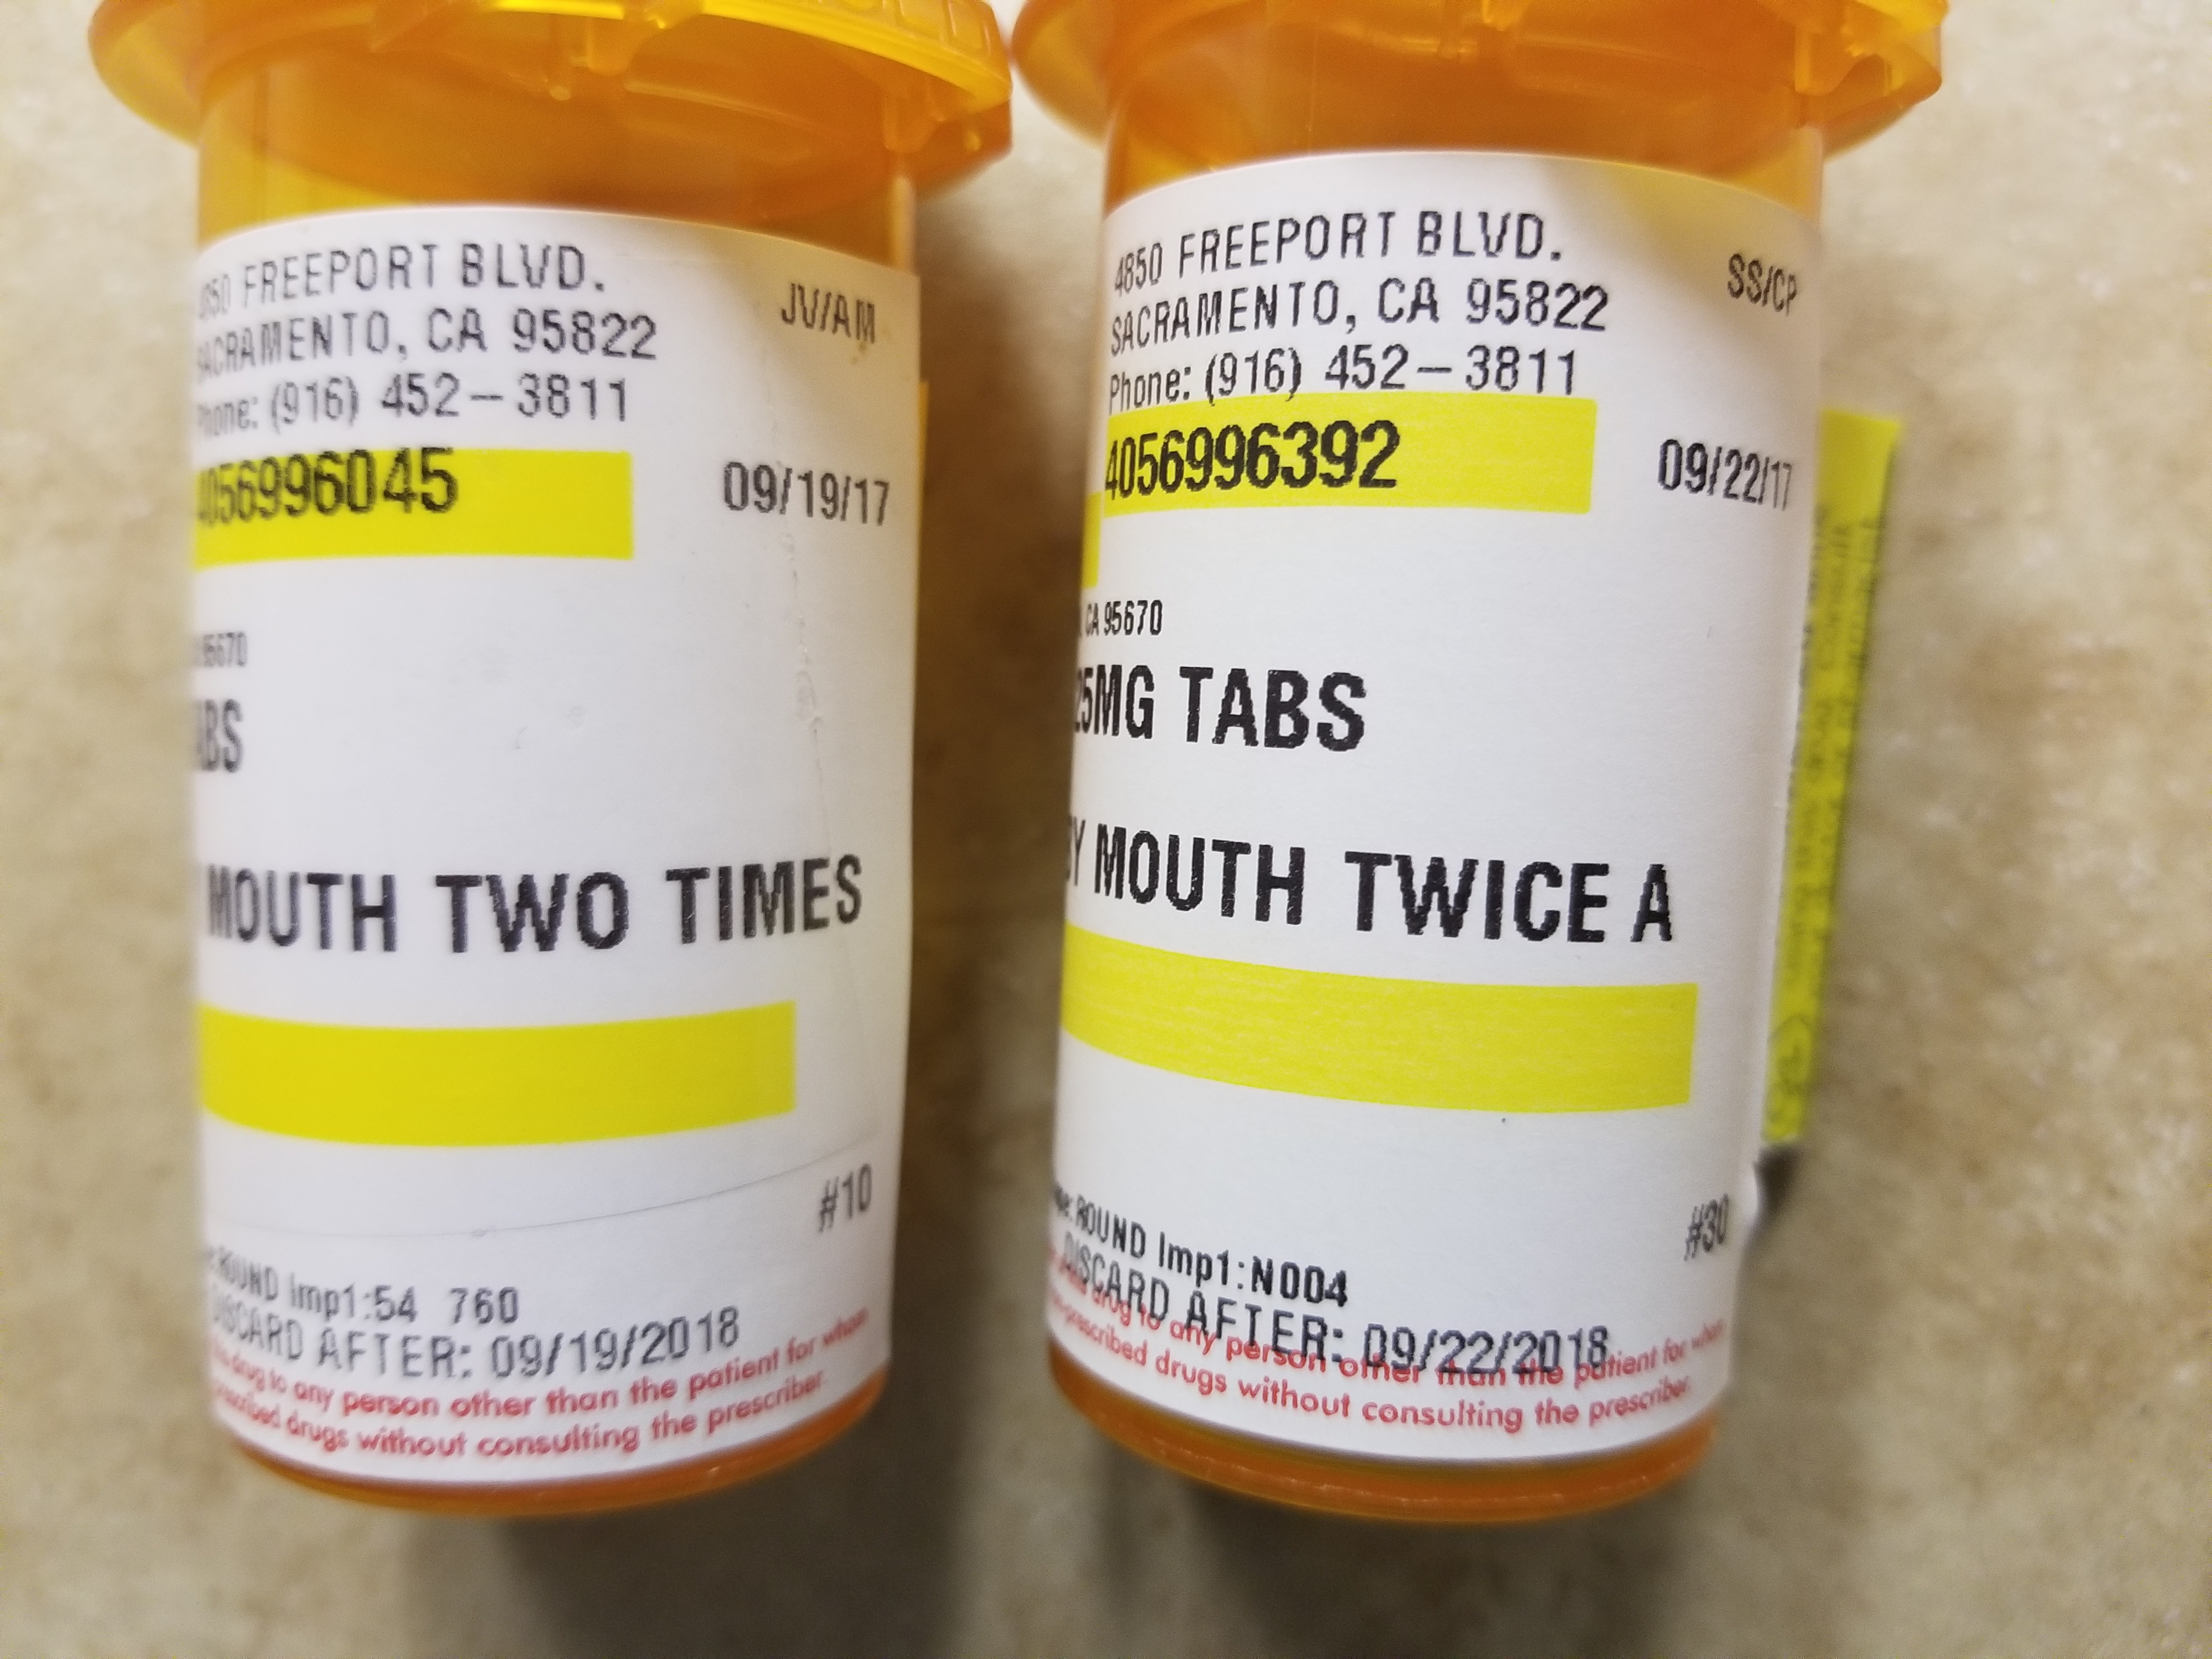
\includegraphics[width=160mm]{proof.jpg}
	\end{figure}
\end{titlepage}
\section*{Section 2.1}
\subsection*{In Exercises 1-16, let the universe be the set $U = \{1, 2, 3, ..., 10\}.$ Let $A = \{1, 4, 7, 10\}$, $B = \{1, 2, 3, 4, 5\}$, and $C = \{2, 4, 6, 8\}.$ List the elements of each.}
\subsubsection*{6: $U - C$}

$U - C = \{1, 3, 5, 9, 10\}$
\subsubsection*{12: $A \cap (B \cup C)$}

$B \cup C = \{1, 2, 3, 4, 5, 6, 8\}$

\fbox{\parbox{\textwidth}{$A \cap (B \cup C) = \{1, 4, 10\}$}}
\subsection*{In exercises 17-24, draw a Venn diagram and shade the given set.}
\subsubsection*{18: $\overline{A} - B$}

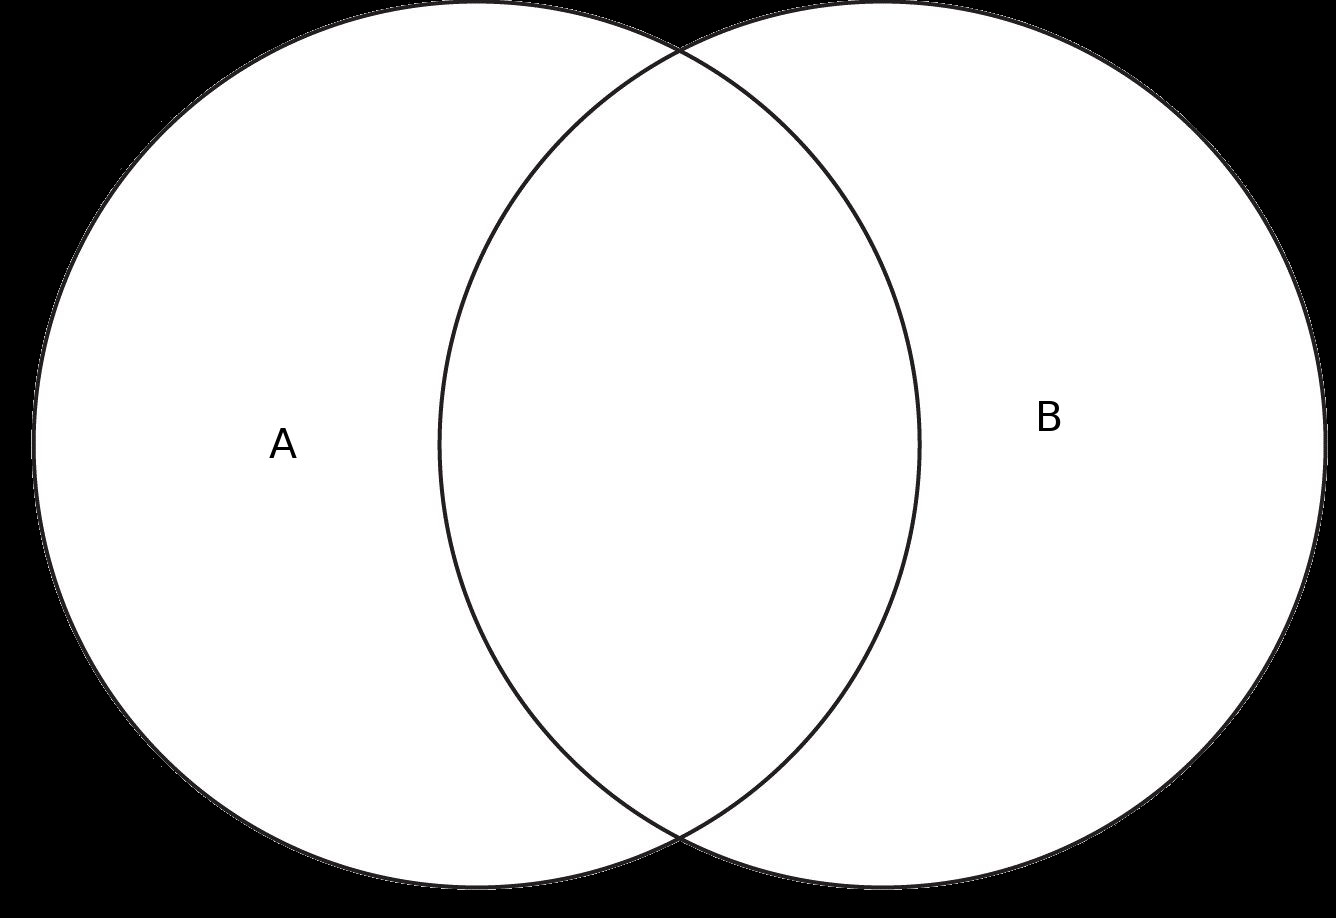
\includegraphics[width=40mm]{notAcomplimentB.jpg}
\subsubsection*{19: $B \cup (B - A)$}

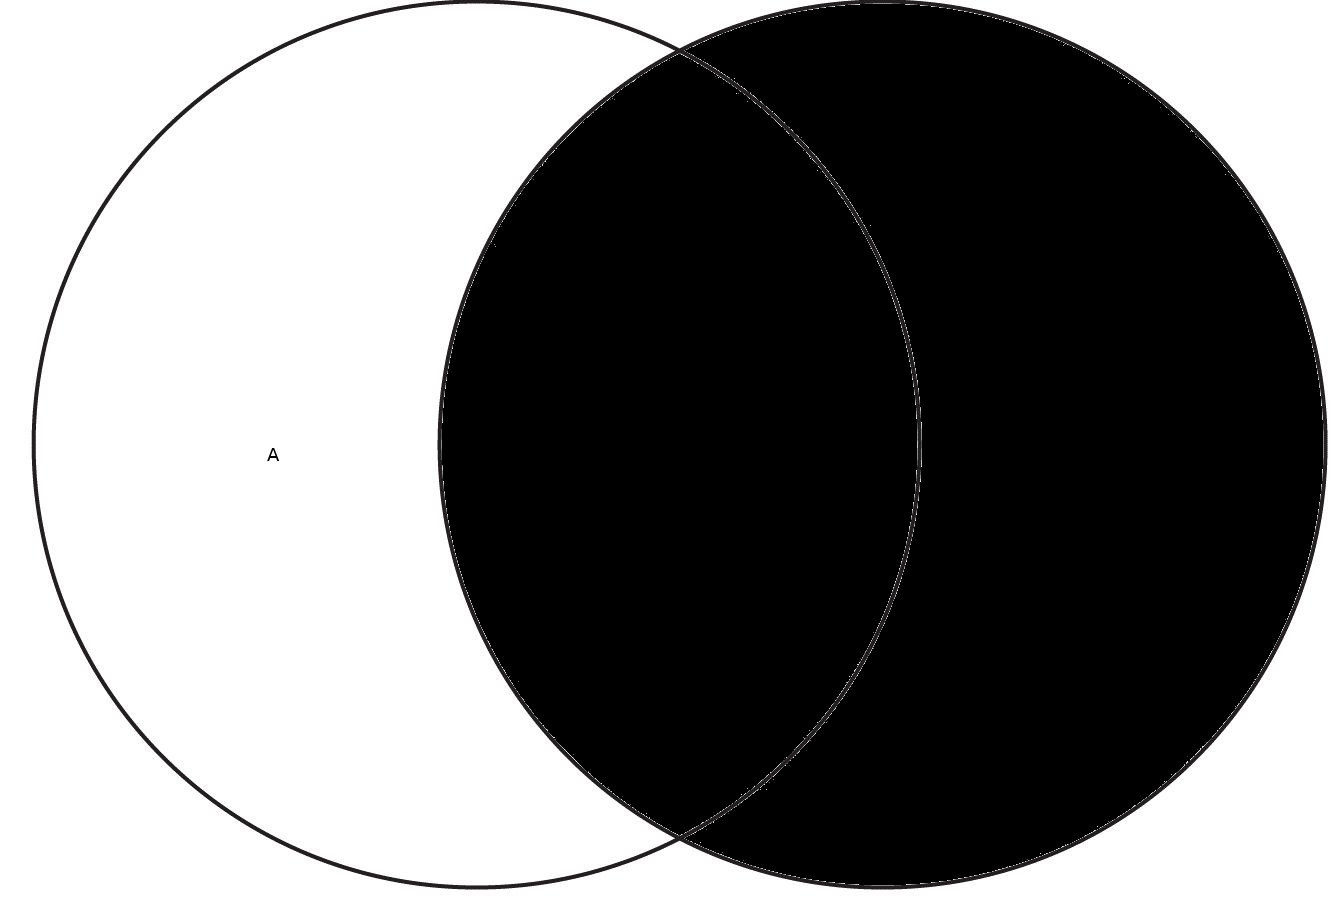
\includegraphics[width=40mm]{number23.jpg}
\subsubsection*{24: $(B - \overline{C}) \cup ((B - \overline{A}) \cap (C \cup B))$}

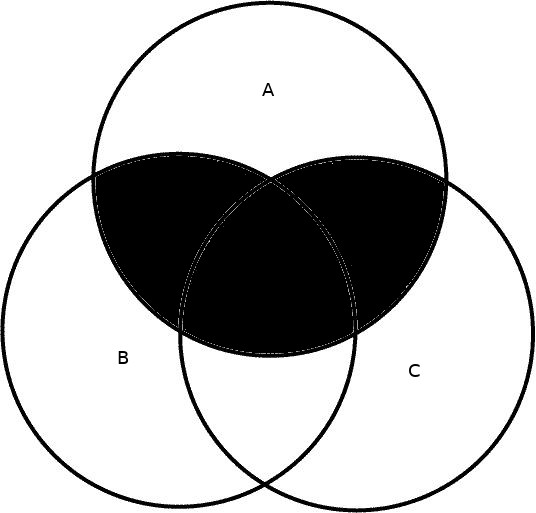
\includegraphics[width=40mm]{number24.jpg}
\subsubsection*{30: A television poll of 151 persons found that 68 watched ``M*E*S*S''; 61 watched ``Leave It to Seaver'' (a base-ball
show), 52 watched ``The Yuppie Hour''; 16 watched both ``M*E*S*S'' and ``Leave It to Seaver''; 25 watched both ``M*E*S*S'' and 
``The Yuppie Hour''; 19 watched both ``Leave It to Seaver'' and ``The Yuppie Hour''; and 26 watched none of these shows. How many 
persons watched all 3 shows?}

Total Number of People: 151

People who didn't watch any of these shows: 26

MESS only: $ 68 - (16 + 25) = 27$

LITS only: $ 61- (16 + 19) = 26$

TYH only: $ 52 - (25 + 19) = 8$

Total people who only watched one show: $8 + 26 + 27 = 61$

Total people who watched exactly two shows: $16 + 19 + 25 = 60$

People who watched 3 shows: (Total People) - \{(No Shows) + (Only One) + (Exactly Two)\}

\fbox{\parbox{\textwidth} {151 - (26 + 61 60) = 4}}
\subsection*{List all partitions of each set}
\subsubsection*{40: $\{1, 2\}$}

\begin{itemize}
	\item $\{\{1\}, \{2\}\}$
	\item $\{\{1, 2\}\}$
\end{itemize}
\subsection*{Determine weather each pair of sets is equal}
\subsubsection*{48: $\{1, 2, 2, 3\}, \{1, 2, 3\}$}

Yes, they are equal, because they contain the same elements. Duplicates don't matter.
\subsubsection*{49: $\{1, 1, 3\}, \{3, 3, 1\}$}

Yes, they are equal. They both contain only a \textit{1} and a \textit{3}
\subsubsection*{53: List the members of $\mathcal{P}(\{a, b, c, d\})$. Which are proper subsets of $\{a, b\}$}

$\mathcal{P}(\{a, b, c, d\})$:
\begin{multicols}{2}
\begin{itemize}
	\item $\{\emptyset\}$
	\item $\{a\}$
	\item $\{b\}$
	\item $\{c\}$
	\item $\{d\}$
	\item $\{a, b\}$
	\item $\{a, c\}$
	\item $\{a, d\}$
	\item $\{b, c\}$
	\item $\{b, d\}$
	\item $\{c, d\}$
	\item $\{a, b, c\}$
	\item $\{a, b, d\}$
	\item $\{a, c, d\}$
	\item $\{b, c, d\}$
	\item $\{a, b, c, d\}$
\end{itemize}
\end{multicols}

Proper Subsets of $\{a, b\}$:
\begin{itemize}
	\item $\{a\}$
	\item $\{b\}$
\end{itemize}

\subsubsection*{54: If \textit{X} has 10 members, how many members does $\mathcal{P}(X)$ have? How many 
proper subsets does \textit{X} have?}

The powerset of \textit{X} has $2^{10}$, or 1024 members.

\textit{X} has 1023 proper subsets
\subsection*{Write \textit{true} if statement is true; otherwise, give a counterexample. The sets $X$, $Y$ and $Z$
are subsets of a universal set $U$. Assume that the universe for Cartesians products is $U * U$}

\subsubsection*{58: $X \cap (Y - Z) = (X \cap Y) - (X \cap Z)$ for all sets $X$, $Y$ and $Z$.}

True
\subsection*{For each condition in Exercises 71--74, what relation must hold between sets $A$ and $B$?}
\subsubsection*{72: $A \cup B = A$}

$B = A$
\subsubsection*{73: $\overline{A} \cap U = \emptyset$}

$A = U$
\end{document}
